% !TeX spellcheck = en_US
% !TEX root = ../thesis-example.tex
%
\chapter{System Setup}
\label{ch:system-setup}

The following section describes the hard- and software components used for the 
thesis and results. All demonstrations have been performed on that environment. 
All dependencies have been explicitly marked to allow a similar, but not exact, 
setup to reproduce these results.

\begin{figure}[htb]
	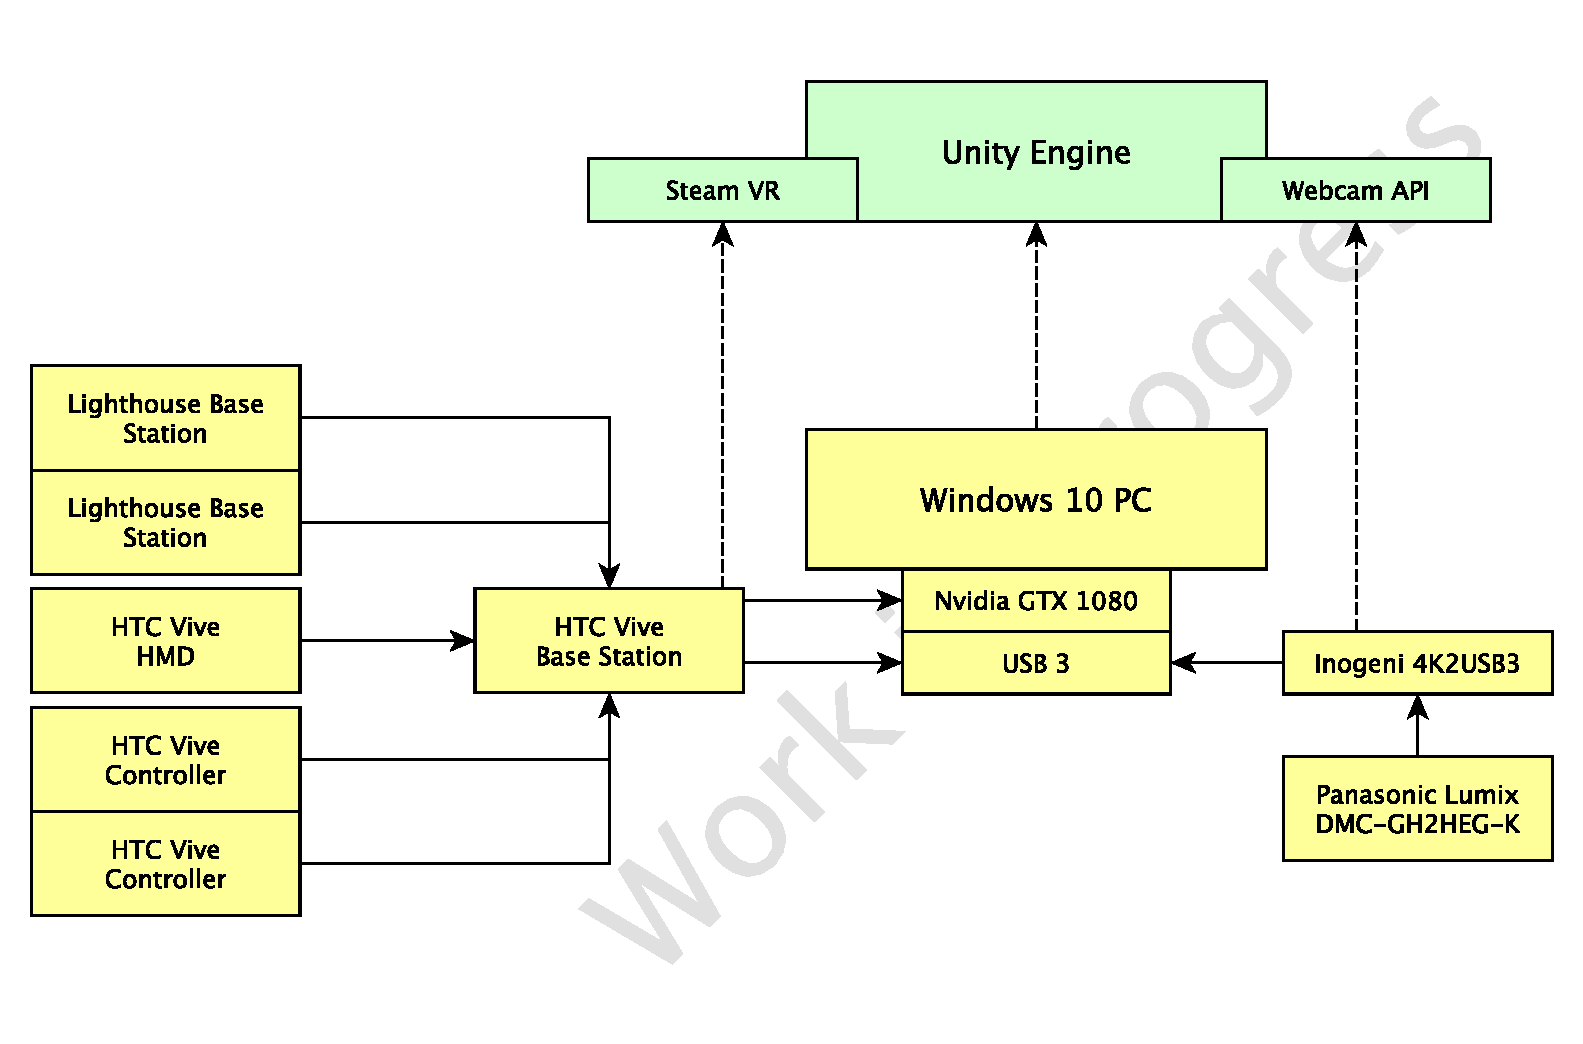
\includegraphics[width=\textwidth]{gfx/System-Components}
	\caption{Diagram of hard- and software components.}
	\label{fig:system-components}
\end{figure}

\section{Hardware Configuration}
\label{sec:hardware-config}

The hardware configuration is split in three main parts:
\begin{my_list}
	\item Windows PC Workstation
	\item Virtual Reality Tracking Solution
	\item Motion Video Input Feed
\end{my_list}

Each individual configuration is basically interchangeable with other systems, 
as long as predefined conditions are met. Each condition is listed first in 
each subsection.

\subsection{PC Workstation}

As the software is built in the Unity Engine, the workstation is limited to 
either Windows or Mac OS X systems the only requirement - besides being 
powerful enough to render the 3D scenes - is two USB3 ports to ensure enough 
data throughput for the video and virtual reality solution, as well as two 
video outputs for a monitor and its headset.
\newline
The configuration used for this thesis is:
\begin{lstlisting}
	CPU: Intel i7-6700 @ 3.40 GHz
	RAM: 16GB DDR4
	GPU: Nvidia Geforce GTX 1080
	System: Windows 10 v. 1703
	Engine: Unity 5.6f3
\end{lstlisting}

This system configuration is to date a high-end workstation that has an 
abundance of render performance and memory for complex and taxing computations 
that have to be performed for a mixed reality composition.

\subsection{Inogeni 4K2USB3 Capture Device}
The Ingoeni 4K2USB3 converter is a standalone box that allows to receive any 
HDMI source and converts it as a webcam video feed usable by "plug'n'play" 
device management of Windows. It's advantage is that it enables any HMDI source 
to be usable as system webcam, thus enabling and arbitrary choice of video 
cameras and a very simple integration with any software through the systems 
provided webcam API. With help of the converter box it's possible to request a 
webcam as video resource and process that video feed as a texture on the GPU.

\subsection{Panasonic GH2 System Camera}
This camera provides a direct video feed via HDMI with low latency. It can 
directly feed into the Inogeni 4K2USB3 and produces a stable, high quality 
video feed with a low signal to noise ratio in well lit environments. 
Additionally it has a well sized photo sensor allowing the camera to capture 
singular frames with reduced motion blur.

\subsection{HTC Vive with Controllers and Lighthouses}
The currently best virtual reality and tracking device available to the public 
is the HTC Vive. It includes two infrared sending stations called "Lighthouse", 
two Vive Controllers\footnote{often delightfully called "Wands" due to its 
controllers design} and a headset. Both, headset and controller systems, are 
enabled with 6 degrees of freedom (6DOF)\todo{6DOF was defined earlier iirc} 
tracking. The tracking system is a black box, in which only the transformation 
matrices for the hand controllers and the HMD can be accessed\footnote{as well 
as sensor input data from the controllers}, which already have been processed 
by the additional SteamVR software. By default this transformation has a 
normalized length of 1 unit to 1 meter. Designing scenery and sense of size is 
therefore rather imaginable. The data provisioning is done by a library called 
"SteamVR for Unity", which makes the usage of said matrices in engine fully 
transparent.

\subsection{Vive Controller Tripod Mount}
Most cameras have a standardized way of mounting tripods. Since the Vive  
controllers have no reference plane. Minuscule differences in mounting angles 
change the projection parameters to noticeable effects, so it was necessary to 
build a mount for the camera to keep controller and video equipment 
transformation synchronized.

\begin{figure}[htb]
	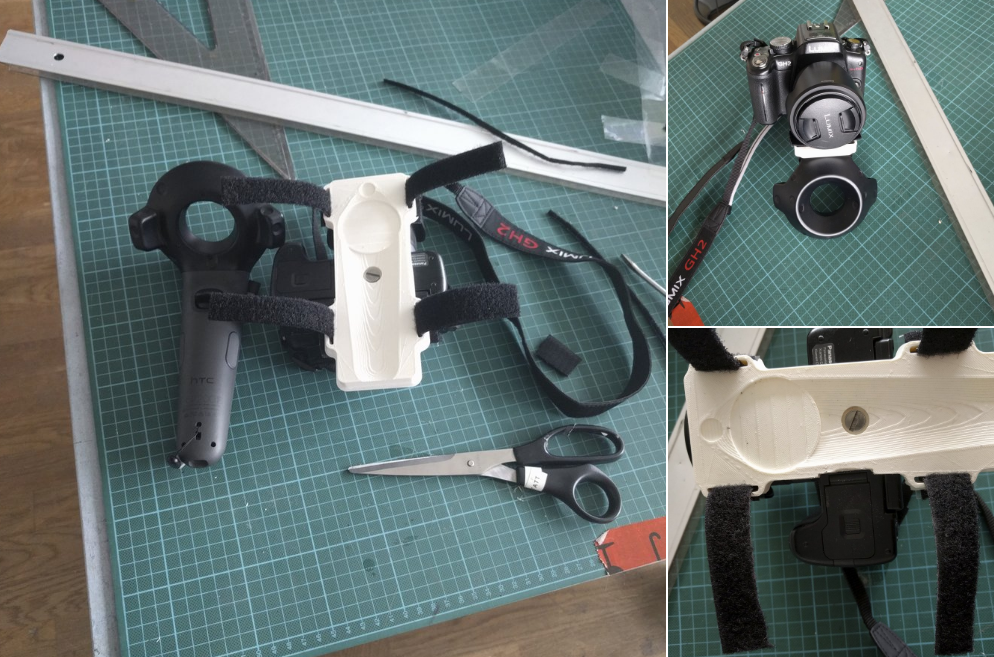
\includegraphics[width=\textwidth]{_raw_resources/ViveStrap-Mount.png}
	\caption{Camera mount for a HTC Vive controller, mounted on the cameras 
		tripod mount}
	\label{fig:system:camera-mount}
\end{figure}

I've built a mount that fits on tripod attachment points and keeps the 
controller locked in the same rotation and position (see figure 
\ref{fig:system:camera-mount}).



\section{Software}

The software of choice is Unity3D, which is a free game engine for students, 
non-profit organizations and small studios. It provides an easy introduction to 
game / 3D engine programming and has a huge development community. While it is 
not the technologically most advanced engine, its fairly easy usage and fast 
development cycles make it a great tool for a bachelor thesis.
\newline
Thankfully, the high abstraction of system APIs means that cross-platform 
development only needs a single code base and makes excruciating tasks like 
webcam access simple - so much so that it boils down to one line of code. 
However, this has drawbacks in overall performance, partially introduced by the 
engine's garbage collection, which are no issue for the used system.
\newline
Its weakness is usually API documentation and - on the downside, too - high 
abstraction levels from most APIs. For example, Unity relies on its own shading 
language which cross-compiles to HLSL, OpenGL and WebGL - this leads to 
problems in buffer and data management, which cannot be controlled well inside 
its render loop.

The software discussed in this thesis integrates and depends additionally on 
SteamVR, a library for Unity, providing the necessary tracking data in the 
engine. SteamVR is developed by Valve, the software is available for free on 
Steam, the complementary library is hosted on GitHub. As of writing this 
thesis, SteamVR is available for Windows and Mac OS X and the software of this 
thesis works on both systems. 

There are no further dependencies or external libraries used.